\section{端侧 Agent Harness：面向受限推理的工作负载闭环}

本赛题关注模型运行时，但实际端侧 Agent 并不是一次性的问答请求。模型需要生成工具调用、等待工具执行、回填观测，再继续生成；如果每一步都重新加载权重，或者把完整终端输出反复塞回上下文，运行时节省下来的内存和 I/O 很快会被编排层重新消耗。为此，SLIM-ARC 增加了一个最小 Agent Harness，把受限内存推理能力接到可复现的工具闭环中。该模块不改变模型计算图，其作用是约束上层请求，使运行时优化在多轮负载中仍然有效。

\subsection{实现路径}

Harness 复用常驻的 OpenAI-compatible HTTP endpoint，执行 \texttt{model $\rightarrow$ shell $\rightarrow$ observation $\rightarrow$ model} 循环。模型只允许返回两种 JSON：\texttt{\{"tool":"shell","args":[...]\}} 或 \texttt{\{"final":"..."\}}。工具参数以 argv 数组传给子进程，不经过 shell 解释器；输出被裁剪后才作为 observation 回填。稳定 system prefix 始终保留，其余消息从最近轮次向前装入字符预算，从源头限制后续 Prefill 的增长。

常驻 endpoint 是正式执行路径。仓库同时保留 \texttt{llama-cli} 兼容入口，便于没有服务端时做功能排查，但该入口每个 Agent step 都可能重新加载模型，因此不用于性能结论。当前实现的边界和指标见表\ref{tab:agent-harness-policy}。

\begin{table}[H]
  \centering
  \small
  \caption{Edge Agent Harness 的端侧约束策略}
  \label{tab:agent-harness-policy}
  \begin{tabular}{p{0.23\textwidth}p{0.34\textwidth}p{0.32\textwidth}}
    \toprule
    端侧问题 & Harness 策略 & 默认边界与可观测量 \\
    \midrule
    重复加载权重
      & 复用常驻 HTTP 模型服务
      & 记录每轮请求耗时；CLI fallback 不作为性能路径 \\
    工具轮次扩大上下文
      & 稳定 prefix + 最近消息窗口；工具观测居中截断
      & context 8192 字符，单次 observation 2048 字符 \\
    Decode 较慢、回答过长
      & 根据已观测的输出速度缩减下一轮 \texttt{max\_tokens}
      & 低于 2.0\,t/s 时乘 0.65；192 tokens 最低降到 48 \\
    工具阻塞或输出爆炸
      & 命令白名单、固定工作目录、超时和输出上限
      & 默认 8\,s、4\,KiB；记录返回码、耗时和截断标志 \\
    多轮失控
      & Agent step 与总墙钟时间双重上限
      & 默认 4 steps、300\,s；超限显式失败 \\
    \bottomrule
  \end{tabular}
\end{table}

\subsection{短上下文与慢输出自适应}

上下文管理采用固定前缀和有界最近窗口。Harness 不做摘要模型调用，也不引入新的常驻内存结构；当消息超过 8192 字符时，优先保留 system prefix 和最近的完整消息，工具输出单独限制在 2048 字符。这样可以给每轮 Prefill 一个确定上界，同时保留最近一次工具结果。

输出预算由上一轮观测驱动。初始上限为 192 tokens；若估算速度低于 2.0\,t/s，下一轮按 0.65 倍收缩，并设置 48 tokens 的下限。这个策略不改变模型采样结果的概率分布，只限制允许生成的最大长度；它适合磁盘缺页或弱 CPU 导致的慢 Decode 场景。若任务确实需要长输出，用户仍可显式提高预算。

\subsection{受限 Shell 与可观测性}

默认命令只包含 \texttt{pwd}、\texttt{uname}、\texttt{df}、\texttt{npu-smi} 等只读诊断操作。Harness 拒绝非白名单程序、绝对路径、\texttt{..} 路径和越出工作目录的符号链接，不使用 \texttt{shell=True}，也不把认证头或环境变量写入指标。每次工具执行均有独立超时和 4\,KiB 输出上限。

运行指标使用 JSONL 记录。模型事件包含上下文字符数、\texttt{max\_tokens}、请求耗时、TTFT、估算输出 token 数与 TPS；工具事件包含 argv、返回码、耗时、输出字符数和截断标志。两类记录可以把“模型慢”与“工具慢”分开，避免把编排等待误归因于推理运行时。

\subsection{功能闭环验证}

图\ref{fig:agent-harness-smoke}是一次确定性本地 smoke 的实际终端记录。测试 endpoint 先返回 \texttt{uname -m} 工具请求，Harness 在受限 shell 中执行并回填观测，第二轮再返回最终答案。首轮估算速度为 1.999\,t/s，触发预算从 192 降到 124，下降 35.4\%；工具返回码为 0，输出未截断。若后续轮次持续低于阈值，预算最多可由 192 降到 48，即上限收缩 75\%。这里验证的是策略闭环和边界是否生效，不是端侧模型的 TPS 加速结果。

\begin{figure}[H]
  \centering
  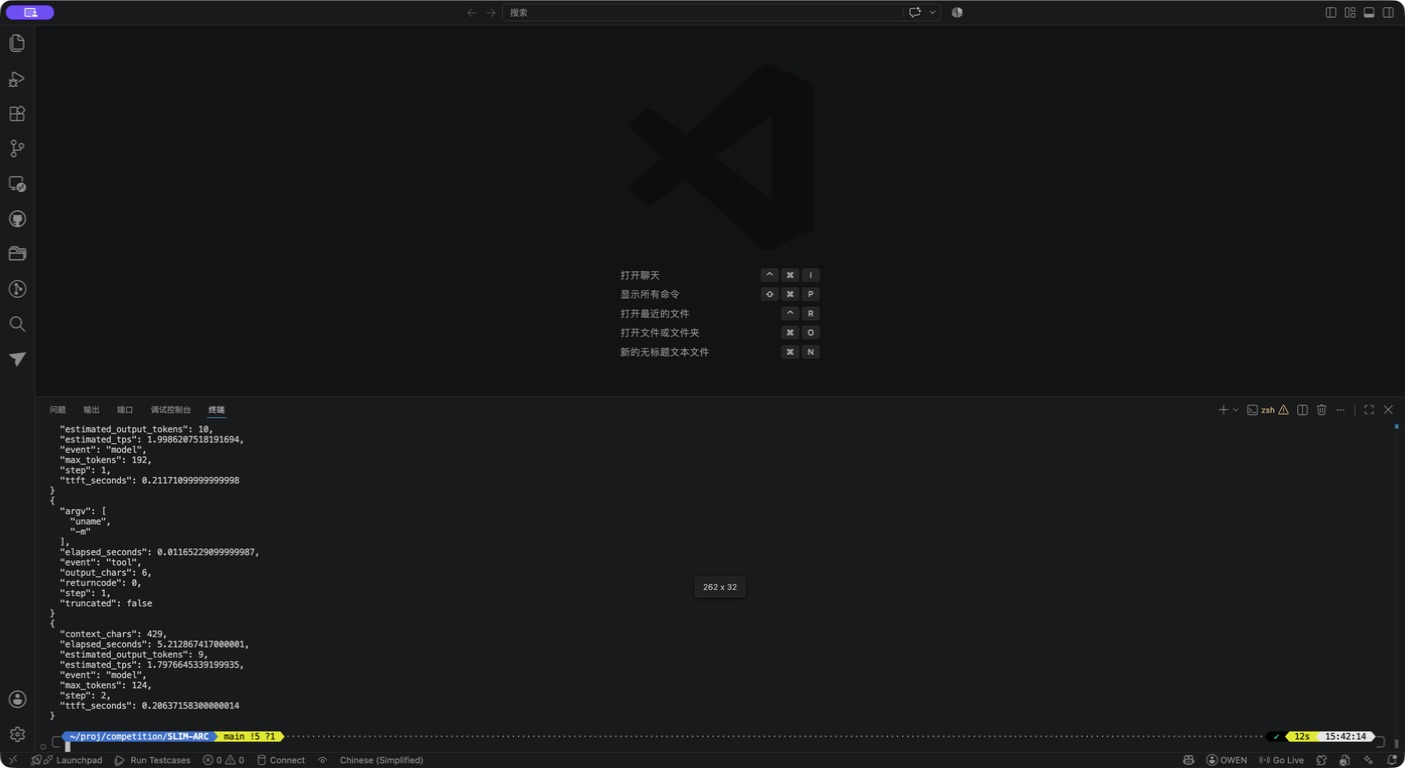
\includegraphics[width=\textwidth]{figures/agent_harness_smoke.png}
  \caption{Agent Harness 确定性 smoke 的实际 JSONL 记录。测试使用本地 OpenAI-compatible SSE endpoint，依次完成模型决策、受限 \texttt{uname -m} 工具调用和最终回答。该图验证工具闭环、指标记录和自适应 token 上限，不代表真实 80B 模型性能。}
  \label{fig:agent-harness-smoke}
\end{figure}

仓库中的 10 个单元测试进一步覆盖上下文裁剪、慢输出预算调整、命令与路径拒绝、输出截断，以及 fake model 驱动的完整闭环。尚未完成固定端侧模型上的 Harness 开/关 A/B，因此本节不宣称 TTFT、TPS 或峰值内存收益。当前可确认的是：运行时负责减少权重与专家访问成本，Harness 负责控制轮数、上下文和输出长度；两者的指标口径已经分开，后续可以在同一设备上做端到端归因。
